\subsection{Twierdzenie \(S_{m,n}\)}
Maszyna \(M\) oblicza \(f^{(k)}(n_1, \dots, n_k) = p\), gdy na słowie 
\(0^{n_1}1\ 0^{n_2} 1 \dots\)
zatrzymuje się z wypisanym \(f^{(k)}(n_1, \dots, n_k)\) na taśmie wyjściowej.

\(f_M^{(k)}\) to funkcja liczona przez maszynę \(M\) o \(k\) argumentach. \\
\(f_m^{(k)}\) to funkcja liczona przez m-tą w numeracji maszynę o \(k\) argumentach.
\begin{theorem}[\(S_{m,n}\)]
    Dla częściowej funkcji rekurencyjnej \(g: \natural^2 \to \natural\) istnieje totalna i~rekurencyjna funkcja \(\sigma: \natural \to \natural\), która spełnia
    \[ g(x,y) = f^{(1)}_{\sigma(x)}(y) \]
\end{theorem}
\begin{proof}
    Niech \(M\) oznacza maszynę, która oblicza \(g\). Konstruujemy maszynę dla \(\sigma(x)\):
    \begin{enumerate}
        \item Wczytaj \(x\).
        \item Skonstruuj maszynę, która przyjmuje \(y\) i symuluje \(x,y\) na \(M\).
        \item Oblicz indeks skonstruowanej maszyny, korzystając z enumeracji częściowych funkcji rekurencyjnych.
    \end{enumerate}
    \vspace{1em}
    \begin{figure}[H]
    \centering
        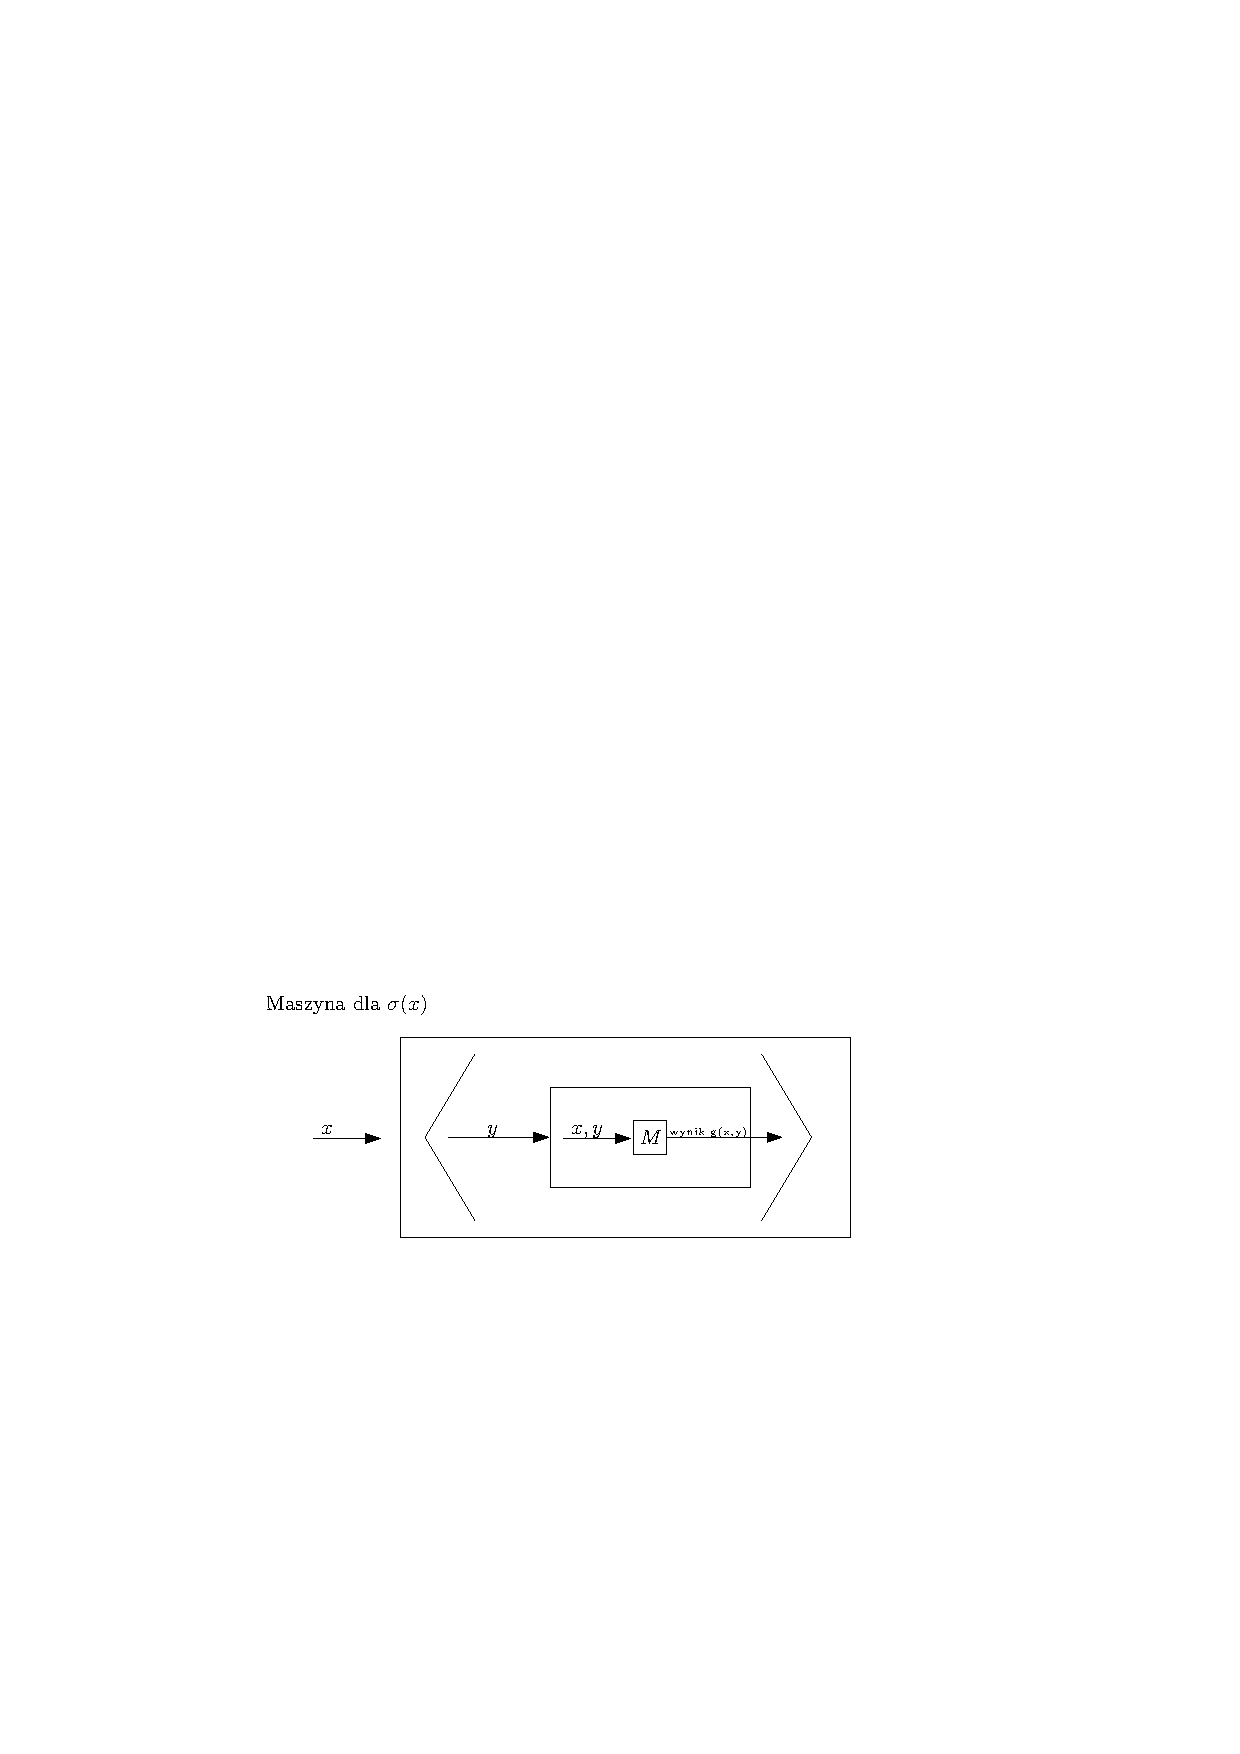
\includegraphics[width=0.6\linewidth]{img/smn.pdf}
    \end{figure}
\end{proof}